\section{The Lifecycle of a Software Update - Centralized vs. Decentralized Approach} \label{appxlifecycle}
In this section, we follow the distinct phases of the lifecycle of a typical software update and discuss the realization in the centralized setting.  This will help the reader to compare with the decentralized software update lifecycle proposed in the main part of the paper. In all the phases, the reader will conclude that the two approaches follow exactly the same logical steps, in order to apply a software update; the essential aspect that differentiates the two approaches is who decides (a central authority vs. the stakeholders community).
 
\subsection{Ideation}
%\paragraph{Centralized approach.}
Traditionally, in the centralized approach, a SU is proposed by some central authority (original author, group of authors, package maintainer etc.), who essentially records the need for a specific SU and then decides when (or, in which version) this could be released. In many cases, (e.g., Bitcoin \cite{bitcoin}, Ethereum \cite{ethereum}) the relevant SU justification document (called BIP, or EIP respectively) is submitted to the community, in order to be discussed. Even when this \say{social alignment} step is included in this phase, the ultimate decision (which might take place at a later phase in the lifecycle), for the proposed SU, is taken by the central authority. Therefore, the road-map for the system evolution is effectively decided centrally. Moreover, this social consensus approach is informal (i.e., not part of a protocol, or output of an algorithm) and is not recorded on-chain as an immutable historical event.

\subsection{Implementation}
In the centralized setting, it is typical (in the context of an open source software development model), when a developer wants to implement a change, first to download from a centrally-owned code repository the version of the source-code that will be the base for the implementation and then, when the implementation is finished, to upload it to the same code repository and submit a \emph{pull-request}. The latter is essentially a call for approval for the submitted code. The central authority responsible for the maintenance of the code-base, must review the submitted code and decide, if it will be accepted, or not. Therefore, in the centralized approach the implementation phase ends with the submission of a pull-request.

\subsection{Approval} \label{appxapproval}
The submitted UP, which as we have seen, is a bundle consisting of source code, metadata and optionally produced binaries, must satisfy certain properties, in order guarantee its \emph{correctness}. Overall, the approver approves the correctness and safety of the submitted UP. We provide a detail list of the properties that a UP must satisfy in order to justify its correctness:

\begin{itemize}
\item
\emph{Correctness and accuracy.} The UP implements correctly (i.e., without bugs) and accurately (i.e., with no divergences) the changes described in the corresponding voted SIP.

\item \emph{Continuity.} Nothing else has changed beyond the scope of the corresponding SIP and everything that worked in the base version for this UP, it continues to work, as it did (as long as it was not in the scope of the SIP to be changed).

\item \emph{Authenticity and safety.} The submitted new code is free of any malware and it is safe to be downloaded and installed by the community; and by downloading it, one downloads the original authentic code that has been submitted in the first place.

\item \emph{Fulfillment of update constraints.} We call the dependencies of an UP to other UPs, the potential conflicts of an UP with other UPs and in general all the prerequisites of an UP, in order to be successfully deployed, \emph{update constraints}. The fulfillment, or not, of all the update constraints for an UP, determines the feasibility of this UP.
\end{itemize}

\begin{figure}[h!] %[H]
    \centering
    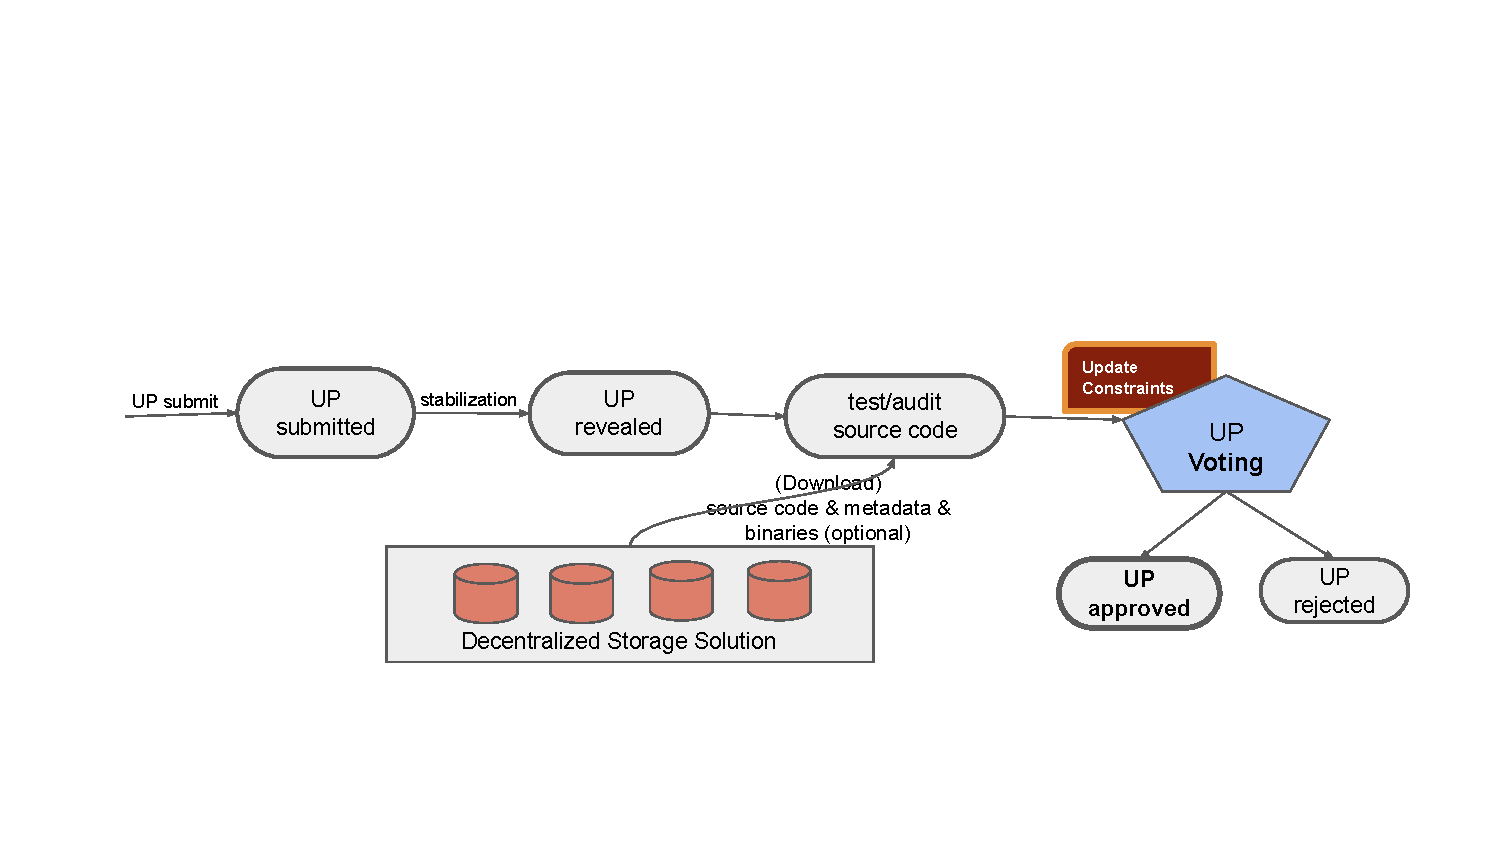
\includegraphics[width=1.0 \columnwidth,keepaspectratio]{figures/approval_phase.pdf}
    \label{figapproval}
    \caption{The approval phase.}
\end{figure}

%\paragraph{Centralized approach.}
From the centralized approach perspective the above properties of the new code that the approver has to verify and approve are not uncommon. In fact, one could argue that these are the standard quality controls in any software development model. The first property has to do with testing; testing that verifies that the changes described in the SIP have been implemented correctly and accurately. In the centralized approach this means that the main maintainer of the code has to validate that the new code successfully passes specific test cases, either by reviewing test results, of executed test cases, or by running tests on his/her own. Regardless, of the testing methodology or type of test employed (unit test, property-based test, system integration test, stress test etc.), this is the basic tool that helps the central authority to decide on the correctness and accuracy of the new code. 

The second property for approving the new code has to do with not breaking something that used to work in the past. In software testing parlance, this is known as regression testing. Again, in the centralized approach, it is the main maintainer's responsibility to verify the successful results of regression tests run against the new code. 

The third property has to do with the security of the new code and the authenticity of the downloaded software. The former calls for the security auditing of the new code. The latter, in the centralized case, is easy. Since, there is a trusted central authority (i.e., the main code maintainer), the only thing that is required, is for this authority to produce new binaries based on the approved source code, sign them and also the source code with his/her private key and distribute the signed code to the community. Then, the users only have to verify that their downloaded source code, or binaries, has been signed by the trusted party and if yes, then to safely proceed to the installation.

Finally, the last property that has to be validated by the approver pertains to the fulfillment of the update constraints. All the prerequisites of an UP must be evaluated and also the potential conflicts triggered by the deployment of an UP must be considered. For example, an UP might be based on a version of the software that has been rejected; or, similarly, it might be based on a version that has not yet been approved. Moreover, it might require the existence of third party libraries that it is not possible to incorporate into the software (e.g., they require licenses, or are not trusted). Then, we have the potential conflicts problem. What if the deployment of an UP cancels a previously approved UP, without this cancellation to be clearly stated in the scope of the corresponding SIP? All these are issues that typically a code maintainer takes into consideration, in order to reach at a decision for a new piece of code.

\subsection{Activation}
%\paragraph{Centralized approach.}
Traditionally, when a software update needs to be activated and it is known that it is likely to cause a chain split, a specific target date, or better, a target block number is set by the central authority, so that all the nodes to get synchronized. Indeed, this is a practice followed by Ethereum \cite{ethereum}. All major releases have been announced enough time before the activation, which takes place when a specific block number arrives (i.e., the corresponding block is mined). All nodes must have upgraded by then, otherwise they will be left behind. In Bitcoin \cite{bitcoin}, there also exists a signaling mechanism\footnote{see BIP-9 at https://github.com/bitcoin/bips/blob/master/bip-0009.mediawiki}. In this case, the activation takes place, only if a specific percentage of blocks (95\%) within a retargeting period of 2016 blocks, signal readiness for the upgrade. 
